\documentclass[11pt]{article}

\usepackage{amsmath, amssymb, amsthm}
\usepackage{tikz}

\theoremstyle{plain}
\newtheorem{thm}{Theorem}[section]
\newtheorem*{thm*}{Theorem}
\newtheorem{prop}[thm]{Proposition}
\newtheorem{lem}[thm]{Lemma}
\newtheorem*{lem*}{Lemma}
\newtheorem{dfn}[thm]{Definition}
\newtheorem{cor}[thm]{Corollary}
\newtheorem{claim}[thm]{Claim}
\newtheorem{conj}[thm]{Conjecture}
\newtheorem{ques}[thm]{Question}
\newtheorem*{rem}{Remark}


\oddsidemargin  0pt
\evensidemargin 0pt
\marginparwidth 40pt
\marginparsep 10pt
\topmargin 0pt
\headsep 10pt
\textheight 8.2in
\textwidth 6.4in
\renewcommand{\baselinestretch}{1.1}

\newcommand{\codeg}{\text{codeg}}
\newcommand{\BBE}{\mathbb{E}}
\newcommand{\BFP}{\mathbf{P}}
\usepackage{amsmath}
\usepackage{amsthm}
\usepackage{amssymb}
\usepackage{mathtools}
\usepackage{hyperref}
\usepackage{url}





\usepackage{graphicx}
\usepackage{caption}
\usepackage{subcaption}

\def\eQb#1\eQe{\begin{eqnarray*}#1\end{eqnarray*}}
\def\eQnb#1\eQne{\begin{eqnarray}#1\end{eqnarray}}
\providecommand{\e}[1]{\ensuremath{\times 10^{#1}}}
\providecommand{\pb}[0]{\pagebreak}
\DeclarePairedDelimiter\ceil{\lceil}{\rceil}
\DeclarePairedDelimiter\floor{\lfloor}{\rfloor}

\newcommand{\E}{\mathrm{E}}
\newcommand{\Var}{\mathrm{Var}}
\newcommand{\Cov}{\mathrm{Cov}}

\def\Qb#1\Qe{\begin{question}#1\end{question}}
\def\Sb#1\Se{\begin{solution}#1\end{solution}}


\newtheoremstyle{quest}{\topsep}{\topsep}{}{}{\bfseries}{}{ }{\thmname{#1}\thmnote{ #3}.}
\theoremstyle{quest}
\newtheorem*{definition}{Definition}
\newtheorem*{theorem}{Theorem}
\newtheorem*{lemma}{Lemma}
\newtheorem*{question}{Question}
\newtheorem*{preposition}{Preposition}
\newtheorem*{exercise}{Exercise}
\newtheorem*{challengeproblem}{Challenge Problem}
\newtheorem*{solution}{Solution}
\newtheorem*{remark}{Remark}
\usepackage{verbatimbox}
\usepackage{listings}
\usepackage{mathrsfs}
\date{}
\title{\vspace{-0.7cm}
Durrett Probability: Problems}

\author{
Youngduck Choi 
\thanks{Department of Mathematics,
}}

\begin{document}

\maketitle

\begin{abstract}
This work contains solutions to some
exercises from Durrett's probability
text.
\end{abstract}


\section{Chapter 6: Markov Chains} \label{sec:MC}

\begin{question}[6.3.3]
\hfill
\begin{figure}[h!]
  \centering
    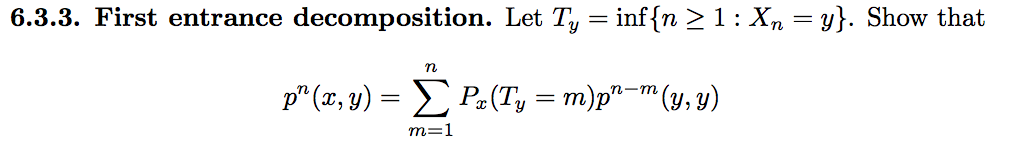
\includegraphics[width=0.7\textwidth]{d-6-3-3.png}
\end{figure}
\end{question}
\begin{solution} \hfill \\
Here we assume countable state space. Observe that
\eQnb
p^{n}(x,y) &=& P_x(X_n = y) = P_x( \bigcup_{m=1}^{n} \{ T_y = m ; X_n = y \}) 
\nonumber \\ 
&=& E_x(1_{\{X_{n - T_y} = y\}} \circ \theta_{T_y} ; T_y \leq n) 
= E_x(E_x( 1_{\{X_{n - T_y} = y\}} \circ \theta_{T_y} | \mathscr{F}_{T_y}) ; T_y \leq 
n) \label{eq:6.3.3.1} \\
&=& E_x( E_{X_{T_y}}(1_{\{X_{n - T_y} = y\}} ; T_y \leq n) 
= E_x(E_y(1_{\{X_{n - T_y}\} });
T_y \leq n) \label{eq:6.3.3.2} \\
&=& \sum_{m=1}^{n} P_x(T_y = m) E_y(1_{\{ X_{n-m} = y\}}) = \sum_{m=1}^{n} P_x(
T_y = m) P^{n-m}(y,y) \nonumber 
\eQne
where~\eqref{eq:6.3.3.1} holds by definition of conditional expectation 
and~\eqref{eq:6.3.3.2} holds by the strong Markov property.  
\end{solution}

\newpage

\begin{question}[6.3.4]
\hfill
\begin{figure}[h!]
  \centering
    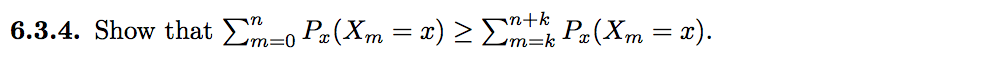
\includegraphics[width=0.7\textwidth]{d-6-3-4.png}
\end{figure}
\end{question}
\begin{solution} \hfill \\
\end{solution}

\newpage

\begin{question}[6.3.5]
\hfill
\begin{figure}[h!]
  \centering
    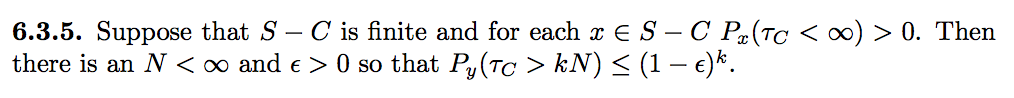
\includegraphics[width=0.7\textwidth]{d-6-3-5.png}
\end{figure}
\end{question}
\begin{solution} \hfill \\
We assume countable state space. Observe that, for any $x \in S \setminus C$,
we can choose $n(x) \in \mathbb{N}$ such that
\eQb
P_x(\tau_C \leq n) > 0.
\eQe
Otherwise, for some $x \in S \setminus C$, by continuity of probability,
\eQb
P_x(\tau_C < \infty) = \lim_{k \to \infty} P_x(\tau_C \leq k) = 0,
\eQe
which is a contradiction. Now, let
\eQb
N = \max_{z \in S \setminus C} n(x). 
\>\>\> \text{and} \>\>\>
\epsilon = \min_{z \in S \setminus C} P_z(\tau_C \leq N).
\eQe
Trivially,
\eQb
P_y(\tau_C > kN) = 0
\eQe
for any $k \in \mathbb{N}$, and $y \in C$, since $y \in C$ implies $\tau_C = 0$ 
by definition. Therefore, it suffices to show 
\eQnb
P_y(\tau_C > kN) \leq (1-\epsilon)^k \label{eq:6.3.5.1}
\eQne
for all $k \in \mathbb{N}$ and $y \in S\setminus C$. Fix $y \in S \setminus C$.
Then,
\eQb
P_y(\tau_C \leq N) &\geq&  \epsilon. 
\eQe
and hence
\eQb
P_y(\tau_C > N) \leq (1-\epsilon)
\eQe
Now, we proceed by induction to prove~\eqref{eq:6.3.5.1}. Suppose, for some $k 
\in \mathbb{N}$ such that $k \geq 2$, 
\eQb
P_y(\tau_C > kN) \leq (1-\epsilon)^k.
\eQe 
We compute
\eQnb
P_y(T_c > (k+1)N) &=& E_y(1_{\{\tau_C > kN \}} \circ \theta_N ; \tau_C > N) 
\nonumber \\
&=& E_y(E_y((1_{\{ \tau_C > kN\} } \circ \theta_N | \mathscr{F}_N); \tau_C > N)) 
\nonumber \\
&=& E_y(E_{X_N}((1_{\{ \tau_C > kN\} }); \tau_C > N)) \label{eq:6.3.5.2} \\
&\leq& E_y(\sup_{z \in S} P_z(\tau_C > kN); \tau_C > N)) \nonumber \\
&\leq& (1-\epsilon)^k E_y(1; \tau_C > N)) = (1-\epsilon)^{k+1} \nonumber  
\eQne
where~\eqref{eq:6.3.5.2} holds by Markov Property, which completes the proof. 
\hfill $\qed$

\end{solution}

\newpage

\begin{question}[6.3.6]
\hfill
\begin{figure}[h!]
  \centering
    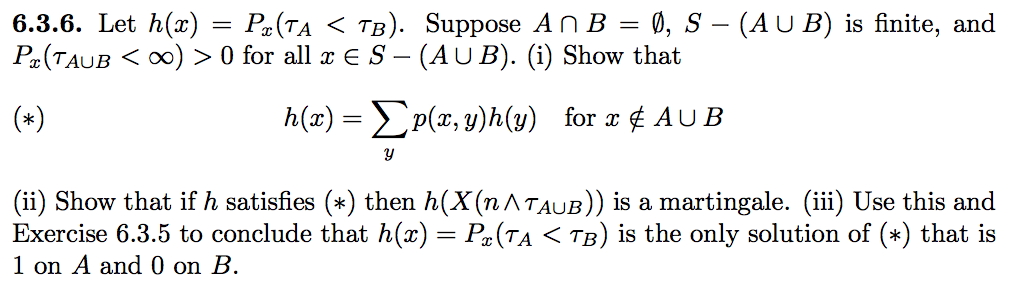
\includegraphics[width=0.7\textwidth]{d-6-3-6.png}
\end{figure}
\end{question}
\begin{solution} \hfill \\
\textbf{(i)}
Let $x \in S \setminus (A \cup B)$. Then,
\eQb
1_{\{\tau_A < \tau_B\}} &=& 1_{ \{ \tau_A < \tau_B \}} \circ \theta_1.
\eQe
It follows that
\eQnb
h(x) &=& P_x(\tau_A < \tau_B) = E_x(1_{\{\tau_A < \tau_B\}}) = 
E_x(1_{\{\tau_A < \tau_B \}} \circ \theta_1) \nonumber \\
&=& E_x(E_x(1_{\{\tau_A < \tau_B \}} \circ \theta_1 | \mathscr{F}_1)) = 
E_x(E_{X_1}(1_{\{ \tau_A < \tau_B \}})) \label{eq:6.3.6.1} \\
&=& \sum_{y} P(X_1 = y)P_y( \tau_A < \tau_B) = \sum_{y} p(x,y) P_y(\tau_A < \tau_B) 
\nonumber  
\eQne
where~\eqref{eq:6.3.6.1} holds by Markov property. 

\bigskip

\textbf{(ii)}


\bigskip


\textbf{(iii)} 

\end{solution}

\newpage


\begin{question}[6.3.7]
\hfill
\begin{figure}[h!]
  \centering
    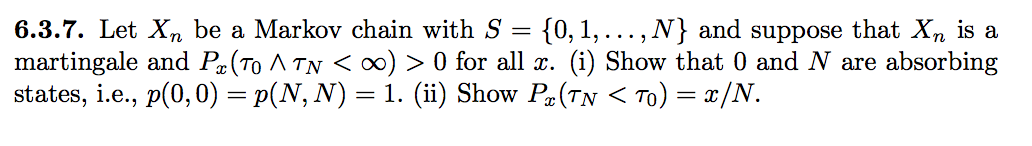
\includegraphics[width=0.7\textwidth]{d-6-3-7.png}
\end{figure}
\end{question}
\begin{solution} \hfill \\
\end{solution}

\newpage

\section{Chapter 2: Law of Large Numbers}


\newpage

\section{Chapter 5: Martingales}

\begin{question}[5.2.1]
\hfill
\begin{figure}[h!]
  \centering
    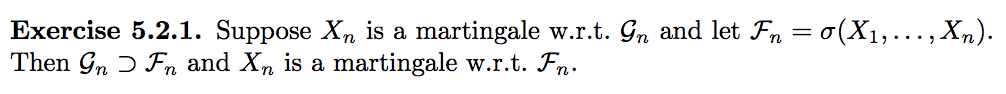
\includegraphics[width=0.7\textwidth]{d-5-2-1.png}
\end{figure}
\end{question}
\begin{solution} \hfill \\
Various properties of conditional expectations are used.

\bigskip

We compute
\eQnb
E[X_{n+1}| \mathscr{F}_n] &=& E[X_{n+1} | \mathscr{G}_{n} | 
\mathscr{F}_n] \label{eq:5.2.1.1} \\
&=& E [X_n| \mathscr{F}_n] \label{eq:5.2.1.2} \\ 
&=& X_n \label{eq:5.2.1.3}  
\eQne
for all $n \in \mathbb{N}$, where~\eqref{eq:5.2.1.1} holds by 
the Tower property,~\eqref{eq:5.2.1.2} holds by Martingale property of $\{G_n\}$
and~\eqref{eq:5.2.1.3} holds by measurability of $X_n$ w.r.t $\mathscr{F}_n$ for 
all $n \in \mathbb{N}$.  \hfill $\qed$
\end{solution}

\newpage

\begin{question}[5.2.2]
\hfill
\begin{figure}[h!]
  \centering
    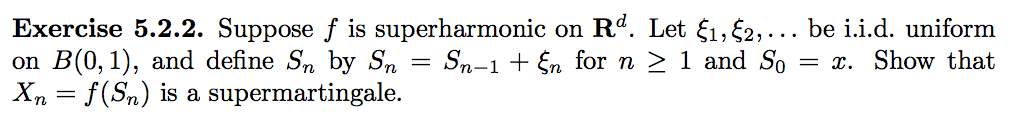
\includegraphics[width=0.7\textwidth]{d-5-2-2.png}
\end{figure}
\end{question}
\begin{solution} \hfill \\
\end{solution}

\newpage

\begin{question}[5.2.3]
\hfill
\begin{figure}[h!]
  \centering
    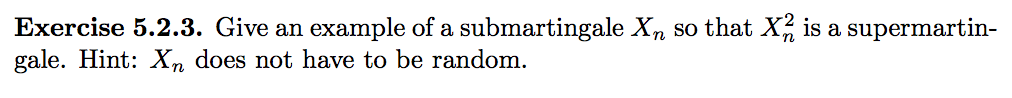
\includegraphics[width=0.7\textwidth]{d-5-2-3.png}
\end{figure}
\end{question}
\begin{solution} \hfill \\
\end{solution}


\end{document}
